\documentclass[11pt,a4paper]{article}
\usepackage[T1]{fontenc}
\usepackage[margin=2.3cm]{geometry}
\usepackage{amsmath,amssymb}
\usepackage{graphicx}
\usepackage[dvipsnames]{xcolor}
\usepackage{enumitem}
\usepackage[colorlinks=true,linkcolor=blue,urlcolor=blue]{hyperref}
\setlength{\parskip}{0.6em}
\setlength{\parindent}{0pt}
\begin{document}

\begin{center}{\LARGE\bfseries openflamevolume}\\[0.4em]{\large Rebuild a 3D flame from many 2D photos using stereo image correlation.}\\[0.2em]\small PAN IIT OSS explainer \textbullet{} higher secondary to advanced undergraduate (levels 4-6)\end{center}

\section*{Why this exists}
A flame is a three-dimensional, glowing object, but every camera records only a flat picture. This explainer follows the idea from one pinhole camera to two cameras (stereo), to matching patches of image by correlation, to several stereo pairs that together rebuild the shape and volume of a flame, and shows how sure we can be of the result.

\section*{The end goal}
Rebuild a 3D flame from many 2D photos using stereo image correlation. The end goal is to turn several views of a flame into its three-dimensional shape and volume, with a number for the uncertainty: to know how disparity gives depth, how correlation finds it, and how many views are enough. The same ideas apply to smoke plumes, deforming solids (digital image correlation) and any surface seen by several cameras.

\section*{How the three sessions build up}
\begin{enumerate}[nosep]
\item \textbf{Session 1: Two eyes see depth} (Level 1 (conceptual interactive model), 60 min).
\item \textbf{Session 2: Find the same spot in two photos} (Level 2 (mathematical engineering model), 75 min).
\item \textbf{Session 3: From many photos to one 3D flame} (Level 3 (simulation and validation), 90 min).
\end{enumerate}

\section{Session 1: Two eyes see depth}

\subsection*{A. Real-world problem}
A flame is a moving 3D object, but a photo of it is flat: every point has only a column and a row. Yet your two eyes find a candle in 3D, because each eye sees it from a slightly different place. How can two cameras do the same and turn two flat photos into the 3D position of the flame tip, in metres? And since a computer finds the match only to a fraction of a pixel, how sure can we be of that number? (General education only: a simplified model, not a measurement procedure.)

\subsection*{B. Concept and theory}
A pinhole camera maps a point (X, Y, Z) in metres, with Z the distance straight ahead, to the pixel x = f X / Z, y = f Y / Z, measured from the image centre. The focal length f is in pixels (lens focal length divided by pixel size). Every point on the same ray through the pinhole lands on the same pixel, so one photo loses the depth. Put a second camera a distance B (the baseline) to the right with the same orientation. The same point appears at x\_L in the left image and x\_R in the right image on the same row, and the difference d = x\_L - x\_R, the disparity, equals f B / Z. Turning this round gives the triangulation formulas Z = f B / d, X = x\_L Z / f, Y = y Z / f. The disparity is found by matching, with an error sigma\_d of a fraction of a pixel. Because dZ/dd = -Z\textasciicircum\{\}2 / (f B), the first-order depth error is sigma\_Z = Z\textasciicircum\{\}2 sigma\_d / (f B): it grows with the square of the distance and falls with a longer baseline or focal length. A Monte Carlo experiment (add random noise to d many times, triangulate each time, measure the spread) checks this formula.

\begin{itemize}[nosep]
\item X, Y, Z: 3D position of a point (Z straight ahead) (m)
\item x, y: pixel position from the image centre (px)
\item f: focal length in pixels (lens focal length / pixel size) (px)
\item B: baseline: distance between the two cameras (m)
\item d: disparity x\_L - x\_R (px)
\item sigma\_d: error of the measured disparity (standard deviation) (px)
\item sigma\_Z: resulting depth uncertainty (m)
\end{itemize}

\begin{equation*}
x = \frac{f\,X}{Z},\qquad y = \frac{f\,Y}{Z}
\end{equation*}

\begin{equation*}
d = x_L - x_R = \frac{f\,B}{Z}
\end{equation*}

\begin{equation*}
Z = \frac{f\,B}{d},\qquad X = \frac{x_L\,Z}{f},\qquad Y = \frac{y\,Z}{f}
\end{equation*}

\begin{equation*}
\sigma_Z \approx \frac{Z^{2}}{f\,B}\,\sigma_d
\end{equation*}

\begin{center}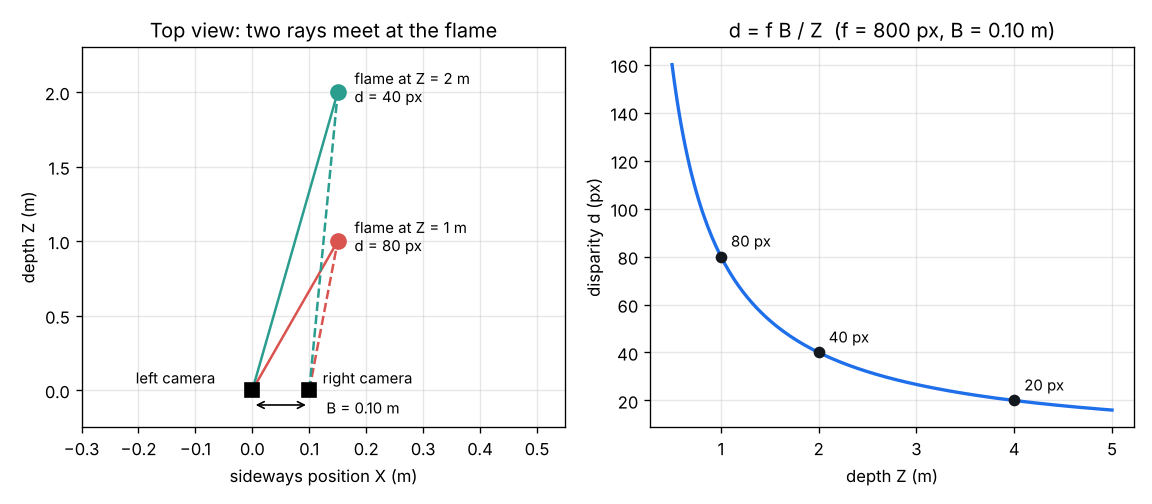
\includegraphics[width=0.85\linewidth]{figures/s01_stereo_geometry.png}\\\small Top view of two cameras and a flame (left) and disparity against depth (right).\end{center}

\subsection*{E. Worked example}
A stereo pair has f = 800 px and B = 10 cm. A flame tip appears at x\_L = 120 px, x\_R = 80 px, row y = 60 px (all from the image centre). Find its 3D position and the depth uncertainty for sigma\_d = 0.5 px. Then find the uncertainty at 4 m.
\begin{enumerate}[nosep]
\item Disparity d = 120 - 80 = 40 px.
\item Depth Z = f B / d = 800 x 0.10 / 40 = 2.00 m.
\item X = x\_L Z / f = 120 x 2.00 / 800 = 0.30 m and Y = y Z / f = 60 x 2.00 / 800 = 0.15 m.
\item Uncertainty sigma\_Z = Z\textasciicircum\{\}2 sigma\_d / (f B) = 2.00\textasciicircum\{\}2 x 0.5 / (800 x 0.10) = 0.025 m = 2.5 cm.
\item At Z = 4 m the same formula gives 16 x 0.5 / 80 = 0.10 m = 10 cm: twice as far, four times the error.
\end{enumerate}
\textbf{Answer.} The flame tip is at (0.30, 0.15, 2.00) m with an uncertainty of 2.5 cm in depth; at 4 m the uncertainty would be 10 cm.

\subsection*{F. Questions}
\begin{enumerate}[nosep]
\item \textbf{Conceptual.} Why can one photo not tell you how far away a flame point is, and why does a second camera fix this?
\item \textbf{Numerical.} f = 1000 px, B = 0.12 m, and a point has disparity d = 60 px and x\_L = 90 px. Find Z and X, and the depth uncertainty for sigma\_d = 0.3 px. Check units and that the answer is reasonable.
\item \textbf{Graph and simulation interpretation.} In the disparity graph (f = 800 px, B = 0.10 m) the disparity is 80, 40 and 20 px at 1, 2 and 4 m. The same 0.5 px error is made at 2 m and at 4 m. Which depth error is larger and by what factor? Explain from the shape of the curve.
\item \textbf{Design and optimisation challenge.} Design: you must measure a flame at Z = 3 m with a depth uncertainty of at most 1 cm. The matching error is 0.5 px and f = 1000 px. What baseline do you need? What if you can double the focal length? Name one practical drawback of a wide baseline.
\end{enumerate}

\section{Session 2: Find the same spot in two photos}

\subsection*{A. Real-world problem}
Session 1 turned a disparity into a depth, but somebody had to say which pixel in the right photo shows the same bit of flame as a pixel in the left photo. A computer must find that match by itself, thousands of times per photo, and to a fraction of a pixel, because a 0.5 px error was already worth 2.5 cm of depth. This is also how digital image correlation (DIC) measures the motion of a speckled surface. How does the computer compare two small patches of image, and how good is the answer on average and in its scatter? (A simplified teaching model on synthetic images.)

\subsection*{B. Concept and theory}
Take a window f from the left image and a window g of the same size from the right. After subtracting each window's mean, the zero-mean normalised cross-correlation is ZNCC = sum (f - mean f)(g - mean g) / sqrt(sum (f - mean f)\textasciicircum\{\}2 x sum (g - mean g)\textasciicircum\{\}2). It is the correlation coefficient of statistics computed over the pixels: +1 for a perfect match, about 0 for unrelated patches, -1 for a negative image. Because means are removed and spreads divided out, a copy with different brightness or contrast (g = a f + b with a > 0) still scores 1. To match, slide the window over whole-pixel shifts s along the same row and keep the best score. The true shift usually lies between two pixels. A parabola through the scores at s - 1, s, s + 1 (c\_minus, c\_0, c\_plus) has its top at delta = (c\_minus - c\_plus) / (2 (c\_minus - 2 c\_0 + c\_plus)), between -0.5 and +0.5 px; the answer is s + delta. Any measurement has a bias (the average error over many repeats) and a spread (the standard deviation of the repeats). The parabola is not the true shape of the score curve, so it pulls answers toward whole pixels (peak locking), a small bias that depends on the sub-pixel part of the shift. Noise adds spread, and a larger window averages noise down, but a window that is too large blurs real detail such as the changing disparity over a curved flame.

\begin{itemize}[nosep]
\item f, g: pixel values in the left and right window (no unit)
\item ZNCC: zero-mean normalised cross-correlation score (no unit)
\item s: trial or measured shift in whole pixels (px)
\item c\_minus, c\_0, c\_plus: scores at s - 1, s, s + 1 (no unit)
\item delta: sub-pixel offset of the parabola top (px)
\item bias, spread: mean error and standard deviation of the error over repeats (px)
\end{itemize}

\begin{equation*}
\mathrm{ZNCC}=\frac{\sum (f-\bar f)(g-\bar g)}{\sqrt{\sum (f-\bar f)^2\,\sum (g-\bar g)^2}}
\end{equation*}

\begin{equation*}
\delta=\frac{c_{-}-c_{+}}{2\,(c_{-}-2c_{0}+c_{+})}
\end{equation*}

\begin{equation*}
\text{bias}=\overline{\hat d-d},\qquad \text{spread}=\operatorname{std}(\hat d-d)
\end{equation*}

\begin{center}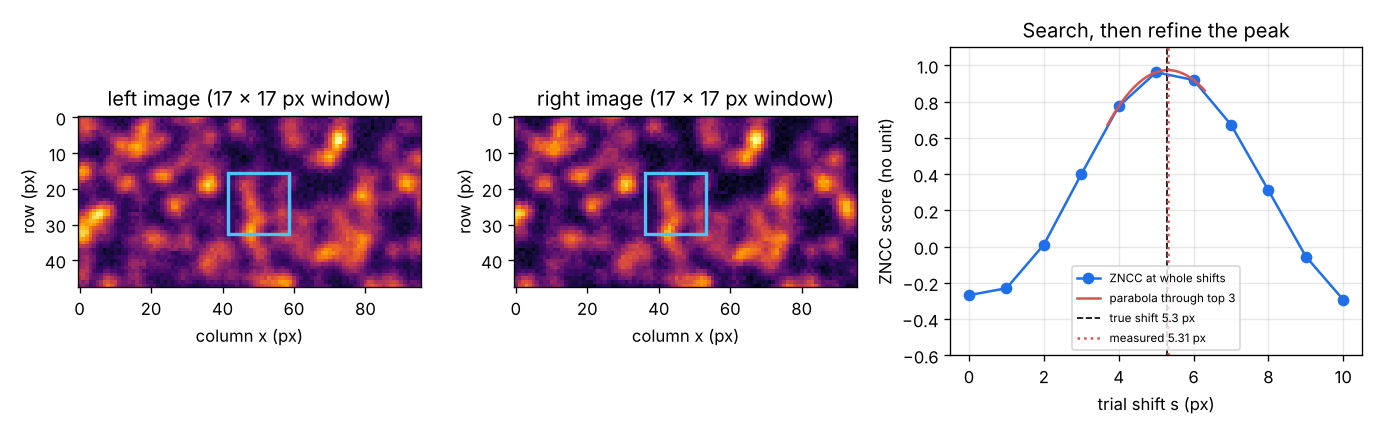
\includegraphics[width=0.85\linewidth]{figures/s02_zncc_match.png}\\\small Two noisy speckle images with the window (left, middle) and the ZNCC score with the parabola refinement (right).\end{center}

\subsection*{E. Worked example}
Compute the ZNCC of f = [2, 4, 6] and g = [11, 12, 13]. Then the scores at disparities 39, 40 and 41 px are 0.80, 0.95 and 0.90. Find the sub-pixel disparity and the depth (f = 800 px, B = 0.10 m), and compare with using d = 40 px.
\begin{enumerate}[nosep]
\item Means: mean f = 4, mean g = 12, so f - mean f = [-2, 0, 2] and g - mean g = [-1, 0, 1].
\item Numerator = 2 + 0 + 2 = 4. Denominator = sqrt(8 x 2) = 4. ZNCC = 1: same pattern, different brightness.
\item delta = (0.80 - 0.90) / (2 (0.80 - 2 x 0.95 + 0.90)) = (-0.10) / (2 x (-0.20)) = +0.25 px.
\item Sub-pixel disparity d = 40 + 0.25 = 40.25 px, so Z = 800 x 0.10 / 40.25 = 1.988 m.
\item Using the whole-pixel d = 40 px would give 2.000 m: rounding the match costs 1.2 cm of depth here.
\end{enumerate}
\textbf{Answer.} ZNCC = 1; the sub-pixel disparity is 40.25 px and Z = 1.988 m, 1.2 cm less than the whole-pixel value.

\subsection*{F. Questions}
\begin{enumerate}[nosep]
\item \textbf{Conceptual.} Why does ZNCC subtract the window mean and divide by the spread, instead of simply summing the squared differences of the pixels?
\item \textbf{Numerical.} Scores at d = 51, 52 and 53 px are 0.70, 0.90 and 0.85. Find the sub-pixel disparity and the depth for f = 800 px and B = 0.10 m. Also find the ZNCC of [1, 3, 5] with [2, 6, 10].
\item \textbf{Graph and simulation interpretation.} In the right panel of Figure 2 (noise 0.06) the spread is 0.95 px for a 7 px window and 0.15 px for a 15 px window. By what factor does it fall? Why not simply use a 50 px window?
\item \textbf{Design and optimisation challenge.} Design: at Z = 2 m with f = 800 px and B = 0.10 m the depth uncertainty must be at most 2 cm. What spread sigma\_d is allowed? With a noise of 0.06, which of the window sizes 7, 11, 15 and 21 px in Figure 2 meet it, and which is the smallest?
\end{enumerate}

\section{Session 3: From many photos to one 3D flame}

\subsection*{A. Real-world problem}
A flame bent by a breeze is neither round nor symmetric, and one stereo pair sees only its front. If several stereo pairs stand around it, match thousands of small windows (Session 2) and triangulate each match (Session 1), we get a cloud of 3D points on the flame surface. Can we turn that cloud into the flame's shape and volume, and show with numbers how close we are to the truth and how many pairs we need? (A simplified teaching model of an opaque, steady, textured surface; not a flame measurement method.)

\subsection*{B. Concept and theory}
The test flame is a sheared elliptic paraboloid: at height z its cross-section is an ellipse with semi-axes a(z) = A0 sqrt(1 - z/H) and b(z) = B0 sqrt(1 - z/H), centred at x = s z (the lean). The area is A(z) = pi A0 B0 (1 - z/H), and adding thin slices (Cavalieri's principle: a sideways shift of a slice does not change its area) gives the exact volume V = pi A0 B0 H / 2. Each stereo pair stands at distance D from the flame axis and looks at it; its two cameras are a baseline B apart. A ray is cast through every pixel, the first hit on the surface gives the texture, and camera noise is added. In the left image a grid of windows is matched along the row of the right image over the disparities the working distance allows (Session 2), then Z = f B / d, X = (col - cx) Z / f, Y = (cy - row) Z / f in the left camera frame, and the point is moved into the world frame. The merged cloud is cut into horizontal slices; in each slice the points are grouped into 24 equal angle sectors, the median radius of each sector gives one corner, and the polygon area comes from the shoelace formula A = 1/2 |sum (x\_i y\_(i+1) - x\_(i+1) y\_i)|. The volume is the sum of slice area times slice thickness. Validation uses two independent checks: the normalised radius rho of each point (rho = 1 on the true surface) and the volume against pi A0 B0 H / 2. Where no camera saw the surface, the polygon cuts straight across the gap, so too few views make the area too small (a bias, not just noise).

\begin{itemize}[nosep]
\item A0, B0, H: semi-axes at the base and height of the flame (m)
\item s: lean (sideways shift per unit height) (no unit)
\item D, B: camera distance from the axis and baseline (m)
\item f: focal length (px)
\item A(z): cross-section area at height z (m\textasciicircum\{\}2)
\item V: flame volume (m\textasciicircum\{\}3)
\item rho: normalised radius of a reconstructed point (1 on the surface) (no unit)
\end{itemize}

\begin{equation*}
A(z) = \pi A_0 B_0\left(1-\frac{z}{H}\right),\qquad V=\int_0^H A(z)\,dz=\frac{\pi A_0 B_0 H}{2}
\end{equation*}

\begin{equation*}
Z=\frac{fB}{d},\quad X=\frac{(c-c_x)Z}{f},\quad Y=\frac{(c_y-r)Z}{f},\quad \mathbf{P}=\mathbf{C}_L+R^{T}(X,Y,Z)^{T}
\end{equation*}

\begin{equation*}
A=\frac12\left|\sum_i \left(x_i y_{i+1}-x_{i+1} y_i\right)\right|,\qquad V\approx\sum_i A_i\,\Delta z
\end{equation*}

\begin{equation*}
\rho=\sqrt{\left(\frac{x-s z}{a(z)}\right)^{2}+\left(\frac{y}{b(z)}\right)^{2}}
\end{equation*}

\begin{center}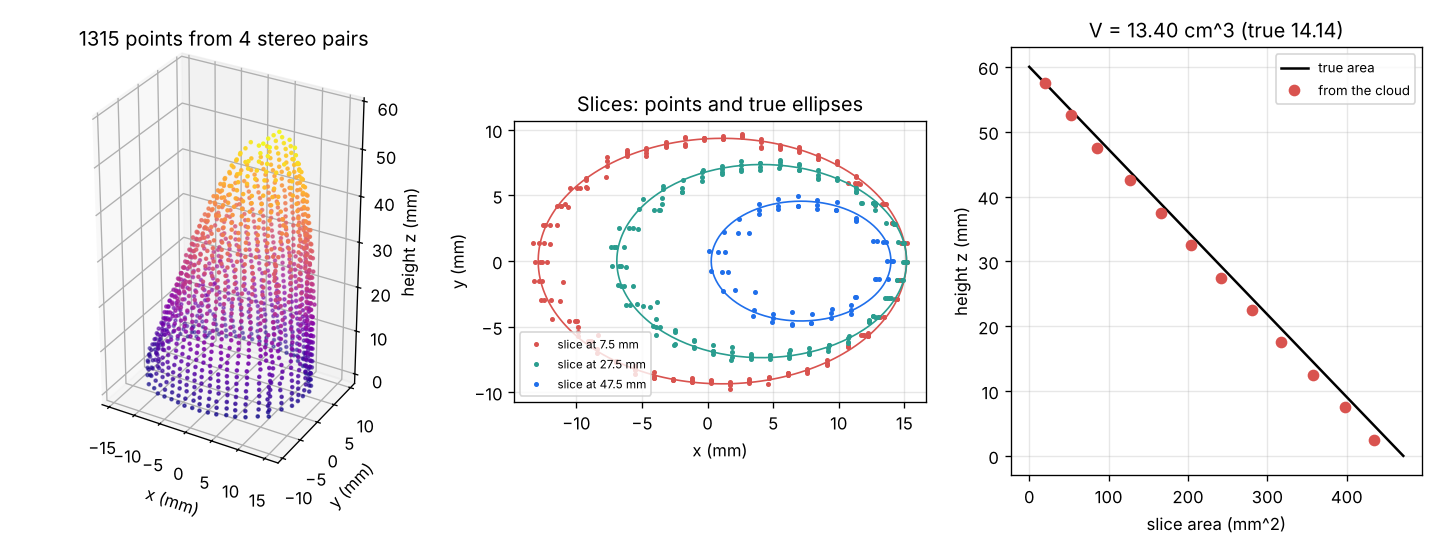
\includegraphics[width=0.85\linewidth]{figures/s03_flame_cloud.png}\\\small Cloud from four stereo pairs, three slices against the true ellipses and slice area against height.\end{center}

\subsection*{E. Worked example}
The test flame has A0 = 15 mm, B0 = 10 mm and H = 60 mm. Find its exact volume and the area of the slice at z = 2.5 mm, and show that 12 slices of 5 mm add up to the exact volume. Then compare the reconstruction from four pairs with it.
\begin{enumerate}[nosep]
\item Exact volume V = pi A0 B0 H / 2 = pi x 15 x 10 x 60 / 2 = 14137 mm\textasciicircum\{\}3 = 14.14 cm\textasciicircum\{\}3.
\item Slice area at z = 2.5 mm: pi x 15 x 10 x (1 - 2.5 / 60) = 471.2 x 0.9583 = 451.6 mm\textasciicircum\{\}2.
\item Midpoints of 12 slices: sum of (1 - (k + 0.5) / 12) over k = 0 to 11 is 12 - 6 = 6, so the sum of areas is 471.2 x 6 = 2827 mm\textasciicircum\{\}2 and the volume is 2827 x 5 = 14137 mm\textasciicircum\{\}3, exact.
\item Reconstruction from four pairs (1315 points): sliced volume 13.40 cm\textasciicircum\{\}3, error 13.40 / 14.14 - 1 = -5.2 percent.
\item The slicing alone, applied to perfect surface points, gives -0.7 percent, so the rest comes from matching: the points lie slightly inside the true surface (median rho - 1 = -0.014, about -2.8 percent in area, because an area goes as rho squared) plus the effect of noise on the median radius.
\end{enumerate}
\textbf{Answer.} The exact volume is 14.14 cm\textasciicircum\{\}3; the four-pair reconstruction gives 13.40 cm\textasciicircum\{\}3 (-5.2 percent), of which only 0.7 percent comes from the slicing method.

\subsection*{F. Questions}
\begin{enumerate}[nosep]
\item \textbf{Conceptual.} A single stereo pair gives 243 points in this simulation, and still the volume is 92 percent too small. Why? What does a second and third pair fix?
\item \textbf{Numerical.} A flame with A0 = 12 mm, B0 = 8 mm and H = 50 mm has the same shape family. Find its exact volume and the exact slice area at z = 25 mm.
\item \textbf{Graph and simulation interpretation.} In Figure 3 the error is -92, -29, -7.0, -5.2 and -4.5 percent for 1, 2, 3, 4 and 6 pairs. Which steps are worth the cost? Why does the curve not reach the dashed line at -0.7 percent?
\item \textbf{Design and optimisation challenge.} Design: a lab can buy 4 cameras (2 pairs) or 6 cameras (3 pairs). The target is a volume within 10 percent. Which do you buy? Also find the depth uncertainty of one pair at D = 0.30 m, B = 0.03 m, f = 1000 px, sigma\_d = 0.5 px.
\end{enumerate}

\section{Real-world mini-project}
\textbf{Choose the number of stereo pairs for a lab burner.} A lab wants to measure the volume of a small bent burner flame with stereo pairs placed evenly around it. Each extra pair costs a camera pair and its synchronisation. Use volume\_study from Session 3 (the test flame, 3 cm baseline, cameras 30 cm from the axis). The lab accepts a volume within 10 percent of the truth. These values are illustrative, not a laboratory procedure.

\section{The path ahead}
\begin{enumerate}[nosep]
\item \textbf{Session 4: Camera calibration from a checkerboard.} A function that finds the focal length and camera pose from the corners of a flat checkerboard seen in a few photos, using a direct linear transform and a least-squares fit.
\item \textbf{Session 5: Cameras that are not parallel: epipolar geometry.} General triangulation from two projection matrices (cameras that toe in towards the flame) and a search along the epipolar line instead of along the image row.
\item \textbf{Session 6: A flickering flame: volume against time.} Render a flame whose height oscillates at 10 Hz, reconstruct the volume frame by frame and find the flicker frequency with a Fourier transform.
\item \textbf{Session 7: The error budget of the whole pipeline.} A Monte Carlo study that adds matching noise, a calibration error and a camera position error and reports the volume uncertainty as a spread.
\item \textbf{Session 8: Rebuild the inside of a translucent flame.} An algebraic reconstruction (ART) of the glow of a translucent, axisymmetric flame from line-of-sight sums seen by at least three directions.
\end{enumerate}

\section{Answers and hints}

\subsection*{Session 1}
\begin{enumerate}[nosep]
\item \textbf{Conceptual.} Hint: What happens to the pixel if you move the point along the ray through the pinhole? Solution: Every point on the ray (X, Y, Z), (2X, 2Y, 2Z), ... lands on the same pixel because x = f X / Z does not change when X and Z are scaled together. So one photo gives only a direction. A second camera at another place gives a second ray, and the two rays meet at only one point, which is the 3D position.
\item \textbf{Numerical.} Hint: Z = f B / d first, then X = x\_L Z / f. Solution: Z = 1000 x 0.12 / 60 = 2.00 m. X = 90 x 2.00 / 1000 = 0.18 m. sigma\_Z = 2.00\textasciicircum\{\}2 x 0.3 / (1000 x 0.12) = 1.2 / 120 = 0.010 m = 1 cm. Units: px x m / px = m. Reasonable: the error is small compared with the 2 m depth.
\item \textbf{Graph and simulation interpretation.} Hint: The curve is steeper at small Z. How many metres does one pixel stand for at each depth? Solution: dZ/dd = Z\textasciicircum\{\}2 / (f B): at 2 m one pixel stands for 4 / 80 = 0.05 m, at 4 m for 16 / 80 = 0.20 m. So at 4 m the error is four times larger (0.5 px gives 2.5 cm at 2 m and 10 cm at 4 m). On a flat part of the curve a small change in d means a large change in Z.
\item \textbf{Design and optimisation challenge.} Hint: Rearrange sigma\_Z = Z\textasciicircum\{\}2 sigma\_d / (f B) for B. Solution: B = Z\textasciicircum\{\}2 sigma\_d / (f sigma\_Z) = 9 x 0.5 / (1000 x 0.01) = 0.45 m. With f = 2000 px, B = 0.225 m. A wide baseline means the two cameras see the flame from quite different directions, so the two images look less alike and matching gets harder; the pair also becomes bulky to mount and calibrate.
\end{enumerate}

\subsection*{Session 2}
\begin{enumerate}[nosep]
\item \textbf{Conceptual.} Hint: Think of two cameras with slightly different exposure. Solution: If one camera is brighter or has more contrast, g = a f + b. A plain sum of squared differences would then be large even for a perfect match. Subtracting the mean removes b and dividing by the spread removes a, so ZNCC stays 1 for any a > 0 and compares only the pattern.
\item \textbf{Numerical.} Hint: delta = (c\_minus - c\_plus) / (2 (c\_minus - 2 c\_0 + c\_plus)). Solution: delta = (0.70 - 0.85) / (2 (0.70 - 1.80 + 0.85)) = (-0.15) / (-0.50) = 0.30 px, so d = 52.30 px and Z = 80 / 52.3 = 1.530 m. For the ZNCC, g = 2 f, which has the same pattern, so ZNCC = 1.
\item \textbf{Graph and simulation interpretation.} Hint: Compute the ratio, then think about what a large window covers on a curved flame. Solution: 0.95 / 0.15 = 6.4, about six times smaller. A very large window covers parts of the flame at different depths, so the disparity is not the same across the window and the match blurs or becomes biased; it also cannot reach near the edge of the flame. The window is a compromise between noise and detail.
\item \textbf{Design and optimisation challenge.} Hint: sigma\_d = sigma\_Z f B / Z\textasciicircum\{\}2. Solution: sigma\_d <= 0.02 x 80 / 4 = 0.40 px. The spreads at noise 0.06 are 0.95, 0.36, 0.15 and 0.10 px, so 11, 15 and 21 px meet it and 11 px (0.36 px) is the smallest, with little margin. (The numbers depend on the synthetic images and the random seeds; the idea does not.)
\end{enumerate}

\subsection*{Session 3}
\begin{enumerate}[nosep]
\item \textbf{Conceptual.} Hint: Ask where the points lie around the flame, not how many there are. Solution: One pair sees only the arc of the surface that faces it, so in each slice the points lie on a short arc and the polygon through them is a thin sliver with almost no area. Adding pairs around the flame fills in the missing arcs, so the polygon follows the whole outline. The number of points matters less than their coverage.
\item \textbf{Numerical.} Hint: V = pi A0 B0 H / 2 and A(z) = pi A0 B0 (1 - z / H). Solution: V = pi x 12 x 8 x 50 / 2 = 7540 mm\textasciicircum\{\}3 = 7.54 cm\textasciicircum\{\}3. A(25) = pi x 12 x 8 x (1 - 0.5) = 150.8 mm\textasciicircum\{\}2, half of the base area 301.6 mm\textasciicircum\{\}2. Units: mm x mm x mm = mm\textasciicircum\{\}3.
\item \textbf{Graph and simulation interpretation.} Hint: Compare the gain of each step, then compare the last value with the dashed line. Solution: Going from 1 to 3 pairs removes 85 points of error, 3 to 6 pairs only 2.5 points more. The curve flattens because coverage is already complete after about three pairs. It stays about 4 points below the dashed line because the remaining error is not about coverage: the matched points lie slightly inside the surface (median rho - 1 is negative) and noise affects the median radius. More cameras cannot remove that; a better matcher or smaller windows could.
\item \textbf{Design and optimisation challenge.} Hint: Compare the 2-pair and 3-pair errors with the target; then use sigma\_Z = D\textasciicircum\{\}2 sigma\_d / (f B). Solution: Two pairs give -29 percent, which misses the target; three pairs give -7.0 percent, which meets it, so buy 6 cameras. The depth uncertainty is 0.30\textasciicircum\{\}2 x 0.5 / (1000 x 0.03) = 0.0015 m = 1.5 mm. Trade-off: more cameras cost more and must be synchronised and calibrated, and a flicker faster than the shutter would spoil the merge. The numbers are for this synthetic flame only.
\end{enumerate}

\section{How to join}
Read \texttt{CONTRIBUTING.md} in the repository, then pick an issue labelled \texttt{good first issue}. Repository: \url{https://github.com/KrunalPanchal1995/pan-iit-oss/tree/main/openflamevolume}

\end{document}
